\section{Présentation de l'existant}

\subsection{Le contrôleur QOPS}

\begin{frame}{Réalisme et efficacité}
    On veut des mouvements réalistes et efficaces
    \begin{itemize}
        \item Optimiser~: choisir le \og{}meilleur\fg{} mouvement parmi tous ceux qui permettent de résoudre la tâche
        %\item Celui qui minimise son coût énergétique et maximise sa vitesse
    \end{itemize}
    \begin{center}
        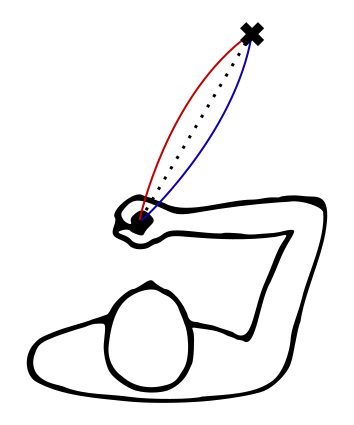
\includegraphics[width=.35\linewidth]{fig/paths}
    \end{center}
\end{frame}

\begin{frame}{Le contrôleur QOPS $[$Rigoux et Guigon 11$]$}
    QOPS présente de bonnes propriétés et on aimerait l'utiliser~:
    \begin{itemize}
        \item Efficace~: trouve le mouvement optimal même en présence de bruit
        \begin{itemize}
            \item Minimise les dépenses énergétiques
            \item Maximise la vitesse
        \end{itemize}
        \item Réaliste~: reproduit les propriétés connues du contrôle moteur humain
    \end{itemize}
%    ~\\
%    Mais~:
%    \begin{itemize}
%        \item il coûte cher en calculs
%        \item on ne peut pas l'utiliser que sur des systèmes simples (bras avec deux articulations seulement)
%    \end{itemize}
\end{frame}

\begin{frame}{Le contrôleur QOPS}
    QOPS permet de contrôler des systèmes mécaniques actionnés par des muscles
    ~\\
    \begin{block}{Pourquoi s'intéresser à un modèle avec muscles~?}
        \begin{itemize}
            \item La robotique s'oriente vers ce type d'actionneurs
            \item Permettent d'avoir des propriétés intéressantes~: réguler la raideur
            \item À terme, profiter de l'énergie cinétique du système avec des muscles élastiques
        \end{itemize}
    \end{block}
\end{frame}

\begin{frame}{Le contrôleur QOPS}
    %Des calculs coûteux~:
    \begin{itemize}
        %\item Utilise une méthode de {\em calcul variationnel} pour trouver le meilleur mouvement pour aller de l'état courant $\jstate$ à l'état désiré $\jstate^*$
        \item Utilise une méthode de {\em calcul variationnel} pour trouver la meilleur commande $\jctrl^*$ qui permet de s'approcher de l'état désiré $\jstate^*$ connaissant l'état courant $\jstate$
        \item État = position et vitesse angulaire des articulations ($\jstate$)
        \item Commande = activations musculaires ($\jctrl$)
    \end{itemize}
    ~\\
    \begin{figure}
        \centering
       % \subfigure{\includegraphics[width=.15\linewidth]{fig/esp_ar}}~~
        \begin{tikzpicture}[scale=1, auto, >=stealth']
    \small

    \tikzstyle{blk} = [rectangle, rounded corners, draw=black, very thick, text width=8cm, minimum height=2cm, text centered]
    \tikzstyle{lab} = [rectangle]
    \tikzstyle{line} = [thick]
    \tikzstyle{connector} = [->,thick]

    %\node [blk] (qopsbox) {$$\jctrl^* = \arg\min_{\discountfactor,t_f} -\rewardfactor~e^{\frac{-t_f.\Delta_t}{\discountfactor}}  + \costfactor~\sum^{t_f}_{t=0} e^{\frac{-t.\Delta_t}{\discountfactor}} \jctrl^2~\Delta_t$$};
    \node [blk] (qopsbox) {$$\jctrl^* = \arg\min_{\jctrl,t_f} \underbrace{\costfactor~\sum^{t_f}_{t=0} \discountfunction(t_f) \jctrl^2~\Delta_t}_\text{coût énergétique} - \underbrace{\rewardfactor~\discountfunction(t_f)}_\text{récompense}$$};
    \node [lab, below of=qopsbox, node distance=1.5cm] (lableqops) {QOPS};

    % Now link the nodes %%%%%%%%%%%%%%%%%%%%%%%%%%%%%%%%%%%%%%%%%%%%%%%%%%%%%%%%%%%%%%%%
    \draw [line]      ($(qopsbox.west) + (0mm,  5mm)$) -- ($(qopsbox.west) + (-5mm,  5mm)$) node[left] {$\jstate$};
    \draw [line]      ($(qopsbox.west) + (0mm, -5mm)$) -- ($(qopsbox.west) + (-5mm, -5mm)$) node[left] {$\jstate^*$};
    \draw [connector] ($(qopsbox.east) + (0mm,  0mm)$) -- ($(qopsbox.east) + ( 5mm,  0mm)$) node[right] {$\jctrl^*$};

\end{tikzpicture}


       % \subfigure{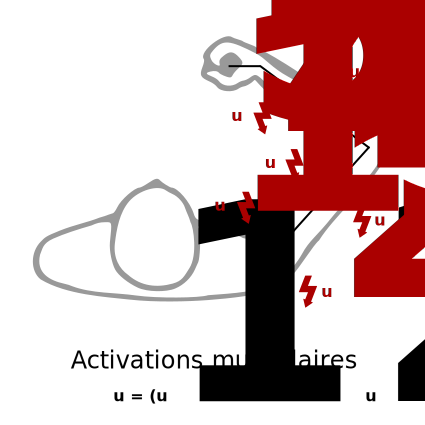
\includegraphics[width=.15\linewidth]{fig/ctrl_u}}
    \end{figure}
    %Compromis vitesse/effort
\end{frame}

\begin{frame}{Le contrôleur QOPS}
    \begin{itemize}
        \item Contrôleur déterministe
        %\item Temps discret
        \item Environnement bruité
        \item Mouvement recalculé à chaque pas de temps
    \end{itemize}
    \begin{figure}
        \centering
        \begin{tikzpicture}[scale=1, auto, >=stealth']
    \small

    % TikZ styles for drawing %%%%%%%%%%%%%%%%%%%%%%%%%%%%%%%%%%%%%%%%%%%%%%%%%%%%%%
    \tikzstyle{block} = [draw,rectangle,thick,minimum height=2em,minimum width=2em]
    \tikzstyle{rounded} = [draw,rectangle,rounded corners=2mm,thick,minimum height=2em,minimum width=2em]
    \tikzstyle{sum} = [draw,circle,inner sep=0mm,minimum size=2mm]
    \tikzstyle{connector} = [->,thick]
    \tikzstyle{line} = [thick]
    \tikzstyle{branch} = [circle,inner sep=0pt,minimum size=1mm,fill=black,draw=black]

    % Node placement with matrix library (3x5 array) %%%%%%%%%%%%%%%%%%%%%%%%%%%%%%%%%%%%
    \matrix[ampersand replacement=\&, row sep=0.2cm, column sep=0.5cm] {

      % row 1
      \node[branch, yshift=-2mm] (b2) {}; \&
      \node[block] (control) {Contrôleur}; \&
      \node[rounded] (noise) {Bruit}; \&
      \node[branch] (b3) {}; \&
      \node[block] (model) {Système mécanique (bras)};
      \\

      % row 2
      \&
      \node[sum] (kalman) {K}; \&
      \&
      \&
      \\

      % row 3
      \&
      \&
      \node[rounded] (delta) {Délai}; \&
      \&
      \node[branch] (b4) {};
      \\
    };

     % Now link the nodes %%%%%%%%%%%%%%%%%%%%%%%%%%%%%%%%%%%%%%%%%%%%%%%%%%%%%%%%%%%%%%%%
     \draw [line]      ($(control.west) + (-1cm, 2mm)$) -- ($(control.west) + (-1cm, 2mm)$) node[left] {$\jstate^*$};
     \draw [line]      (b2) -- ($(control.west) + (-1cm, -2mm)$) node[left] {$\jstate_0$};
     \draw [connector] ($(control.west) + (-1cm, 2mm)$) -- ($(control.west) + (0, 2mm)$);
     \draw [connector] (b2) -- ($(control.west) + (0, -2mm)$);
     \draw [connector] (control) -- node {$\jctrl$} (noise);
     \draw [line]      (noise) -- node {$\tilde{\jctrl}$} (b3);
     \draw [connector] (b3) -- (model);
     \draw [connector] (b3) |- (kalman);
     \draw [line]      (model) -- node {$\jstate_{t+1}$} (b4);
%     \draw [connector] (b4) -- ++(2.5cm,0) -- ++(0,3cm) -- ++(-2.5cm,0) -- node {$\jstate_t$} (model.north);
     \draw [connector] (b4) -- (delta);
     \draw [connector] (delta) -| (kalman);
     \draw [line]      (kalman) -| node[pos=0.20] {$\tilde{\jstate}$} (b2);

\end{tikzpicture}

    \end{figure}
\end{frame}

\subsection{Les limites de QOPS}

\begin{frame}{Les limites de QOPS}
    QOPS génère des mouvements efficaces et réalistes mais\dots
    \begin{itemize}
        \item On ne peut pas l'utiliser sur autre chose que des systèmes simples (bras avec deux articulations)
        \item Les méthodes de calcul variationnel coûtent chères en calculs
    \end{itemize}
\end{frame}

\begin{frame}{Les causes de ces limites~?}
    \begin{small}
        Le temps nécessaire pour trouver le meilleur mouvement augmente exponentiellement avec~:
        \begin{itemize}
            \item La taille du vecteur d'état
            \item La taille du vecteur de commande
        \end{itemize}
        \begin{block}{QOPS}
            \begin{itemize}
                \item Définit l'état dans l'espace articulaire ($\jstate$)
                \item Définit la commande dans l'espace des activations musculaires ($\jctrl$)
            \end{itemize}
        \end{block}
        \begin{block}{Conséquence}
            Ajouter une articulation au modèle contrôlé par QOPS augmente la taille de
            ces deux vecteurs et allonge considérablement la durée des calculs
        \end{block}
    \end{small}
\end{frame}

%%%%%%%%%%%%%%%%%%%%%%%%%%%%%%%%%%%%%%%%%%%%%%%%%%%%%%%%%%%%%%%%%%%%%%%%%%%%%%%

\section{Une nouvelle architecture}

\subsection{Découpage du problème initial}

\begin{frame}{Objectifs}
    On aimerait
    \begin{itemize}
        \item Conserver les propriétés intéressantes de QOPS (mouvement réaliste et efficace)
        \item Travailler sur des systèmes avec beaucoup d'articulations
        \item Sans pour autant augmenter la taille des vecteurs d'état et de commande
    \end{itemize}
\end{frame}

\begin{frame}{Reformulation du problème}
    Par chance, le problème du contrôle moteur peut être décrit dans différents espaces~:
    \begin{block}{Vecteur d'état}
        \begin{figure}
            \centering
            \subfigure{\includegraphics[width=.25\linewidth]{fig/esp_ar}}~~
            \subfigure{\includegraphics[width=.25\linewidth]{fig/esp_op}}
        \end{figure}
    \end{block}
\end{frame}

\begin{frame}{Reformulation du problème}
    %Par chance, le problème du contrôle moteur peut être décrit dans différents espaces~:
    \begin{block}{Vecteur des commandes}
        \begin{columns}
            \begin{column}{0.40\textwidth}
                Agir à plusieurs niveaux~:
                \begin{itemize}
                    \item Cinématique
                    \item Dynamique
                    \item Actionnement
                \end{itemize}
            \end{column}
            \begin{column}{0.50\textwidth}
                Définie dans différents espaces~:
                \begin{itemize}
                    \item Espace de la tâche
                    \item Espace articulaire
                    \item Espace des activations
                \end{itemize}
            \end{column}
        \end{columns}
        \begin{figure}
            \centering
            \subfigure{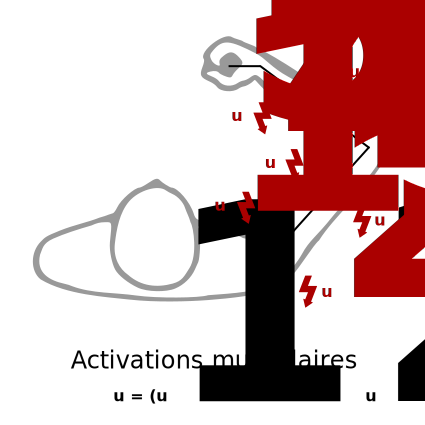
\includegraphics[width=.25\linewidth]{fig/ctrl_u}}~~
            \subfigure{\includegraphics[width=.25\linewidth]{fig/ctrl_tau}}
            \subfigure{\includegraphics[width=.25\linewidth]{fig/ctrl_phi}}
        \end{figure}
    \end{block}
\end{frame}

%\begin{frame}{Bilan}
%    On aimerait {\em optimiser} (calculer la meilleure trajectoire) dans l'{\em espace de
%    la tâche} quel que soit le nombre d'articulations du système
%\end{frame}

\begin{frame}{Idée}
    \begin{figure}
        \centering
        \begin{tikzpicture}[scale=1, auto, >=stealth']
    \small

    \tikzstyle{blk} = [rectangle, rounded corners, draw=black, very thick, text width=8cm, minimum height=2cm, text centered]
    \tikzstyle{lab} = [rectangle]
    \tikzstyle{line} = [thick]
    \tikzstyle{connector} = [->,thick]

    \node [blk] (qopsbox) {Planifie les activations musculaires $\jctrl$ pour tout le mouvement};
    \node [lab, below of=qopsbox, node distance=1.5cm] (lableqops) {QOPS};

    % Now link the nodes %%%%%%%%%%%%%%%%%%%%%%%%%%%%%%%%%%%%%%%%%%%%%%%%%%%%%%%%%%%%%%%%
    \draw [line]      ($(qopsbox.west) + (0mm,  5mm)$) -- ($(qopsbox.west) + (-5mm,  5mm)$) node[left] {$\jstate$};
    \draw [line]      ($(qopsbox.west) + (0mm, -5mm)$) -- ($(qopsbox.west) + (-5mm, -5mm)$) node[left] {$\jstate^*$};
    \draw [connector] ($(qopsbox.east) + (0mm,  0mm)$) -- ($(qopsbox.east) + ( 5mm,  0mm)$) node[right] {$\jctrl^*$};

\end{tikzpicture}


    \end{figure}
    \begin{figure}
        \centering
        \input{tikz/tikz_qopslqp.tex}
    \end{figure}
\end{frame}

%\begin{frame}{Idée}
%        %Planifier la trajectoire dans l'espace de la tâche
%        Définir l'état et la commande dans l'espace de la tâche
%        %\begin{itemize}
%        %    \item Définir l'état dans l'espace de la tâche ($\ostate$)
%        %    \item Définir la commande dans l'espace de la tâche ($\octrl$)
%        %\end{itemize}
%        \begin{figure}
%            \centering
%            \subfigure{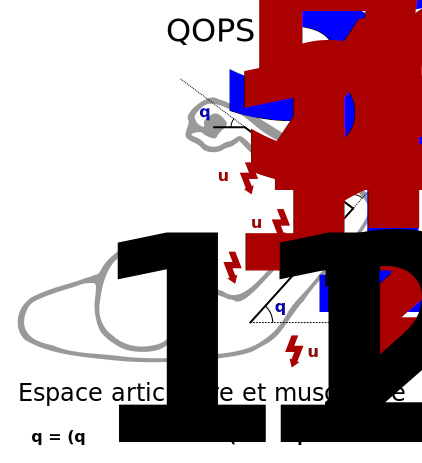
\includegraphics[width=.25\linewidth]{fig/qops}}~~$\Rightarrow$~~
%            \subfigure{\includegraphics[width=.25\linewidth]{fig/qopslqp}}
%        \end{figure}
%\end{frame}

%\begin{frame}{Méthode}
%    \begin{block}{Comment~?}
%        Traduire la dynamique du système dans l'espace de la tâche $[$Kathib 87$]$
%        \begin{small}
%            \begin{align*}
%                \vs{F} & = m \vs{a} \\
%                \vt - \vs{n}(\q, \dq)  & = \ms{M}(\q) ~ \ddq \\
%                \ddq & = \ms{M}^{-1}(\q) ~ \vt -  \ms{M}^{-1}(\q) ~ \vs{n}(\q, \dq) \\
%                     & \dots \\
%                \ddx & = \jacobian(\q) ~ \ms{M}^{-1}(\q) ~ \jacobian^T(\q) ~ \octrl - \jacobian(\q) ~ \ms{M}^{-1}(\q) ~ \vs{n}( \q, \dq ) + \djacobian(\q, \dq) ~ \dq
%            \end{align*}
%            %En utilisant $\dx = \jacobian(\q)\dq$ et $\vt = \jacobian^T(\q) ~ \octrl$
%        \end{small}
%    \end{block}
%\end{frame}

%%%%%%%%%%%%%%%%%%%%%%%%%%%%%%%%%%%%%%%

\subsection{Optimisation du mouvement dans l'espace opérationnel}

\begin{frame}{Optimisation du mouvement dans l'espace opérationnel}
    \begin{itemize}
        \item On utilise $\qopsx$ pour planifier la trajectoire optimale dans l'espace opérationnelle
        \item Modifie la dynamique utilisée pour se projeter à l'état suivant
        \item Dynamique traduite dans l'espace de la tâche $[$Kathib 87$]$
    \end{itemize}
    \begin{figure}
        \centering
        \begin{tikzpicture}[scale=1, auto, >=stealth']
    \small

    \tikzstyle{blk} = [rectangle, rounded corners, draw=black, very thick, text width=3.5cm, minimum height=2cm, text centered]
    \tikzstyle{lab} = [rectangle]
    \tikzstyle{connector} = [->,thick]
    \tikzstyle{line} = [thick]

    \node[blk] (boxB1) {Optimisation de la dynamique dans l'espace de la tâche}; \&
    \node [lab, below of=boxB1, node distance=1.5cm] (lableqops) {$\qopsx$};

    % Now link the nodes %%%%%%%%%%%%%%%%%%%%%%%%%%%%%%%%%%%%%%%%%%%%%%%%%%%%%%%%%%%%%%%%
    \draw [line]      ($(boxB1.west) + (0mm,  5mm)$) -- ($(boxB1.west) + (-5mm,  5mm)$) node[left] {\dontforget{$\ostate$}};
    \draw [line]      ($(boxB1.west) + (0mm, -5mm)$) -- ($(boxB1.west) + (-5mm, -5mm)$) node[left] {\dontforget{$\ostate^*$}};
    \draw [connector] ($(boxB1.east) + (0mm,  0mm)$) -- ($(boxB1.east) + ( 5mm,  0mm)$) node[right] {\dontforget{$\octrl^*$}};

\end{tikzpicture}

    \end{figure}
%    \begin{footnotesize}
%        \begin{block}{Nouvelle fonction de processus (dynamique du système)}
%            \begin{equation*}
%                \processfuntion(\ostate, \octrl) = \begin{pmatrix}
%                                                       \jacobian(\q) ~ \ms{M}^{-1}(\q) ~ \jacobian^T(\q) ~ \octrl - \jacobian(\q) ~ \ms{M}^{-1}(\q) ~ \vs{n}( \q, \dq ) + \djacobian(\q, \dq) ~ \dq \\
%                                                       \dx
%                                                   \end{pmatrix} \label{eq:process-function}
%            \end{equation*}
%        \end{block}
%    \end{footnotesize}
\end{frame}

%%%%%%%%%%%%%%%%%%%%%%%%%%%%%%%%%%%%%%%

\subsection{Optimisation du mouvement dans l'espace des muscles}

\begin{frame}{Optimisation du mouvement dans l'espace des muscles}
    \begin{small}
        \begin{block}{Exécuter le mouvement}
            Calculer les activations musculaires $\jctrl$ permettant d'exécuter la force $\octrl^*$
        \end{block}
        ~\\
        Muscles = système d'actionnement redondant
        \begin{itemize}
            \item Plusieurs solutions
            \item On veut optimiser $\Rightarrow$ trouver la meilleure solution
        \end{itemize}
    \end{small}
    \begin{figure}
        \centering
        \begin{tikzpicture}[scale=1, auto, >=stealth']
    \small

    \tikzstyle{blk} = [rectangle, rounded corners, draw=black, very thick, text width=3.5cm, minimum height=2cm, text centered]
    \tikzstyle{lab} = [rectangle]
    \tikzstyle{connector} = [->,thick]
    \tikzstyle{line} = [thick]

    % Node placement with matrix library (3x2 array) %%%%%%%%%%%%%%%%%%%%%%%%%%%%%%%%%%%%
    \matrix[ampersand replacement=\&, row sep=0.3cm, column sep=1cm] {
        % row 1
        %\node[blk] (boxB1) {Optimisation de la dynamique dans l'espace de la tâche}; \&
        %\node[blk] (boxB2) {Optimisation des activations dans l'espace articulaire}; 
        \node[blk, fill=gray!20] (boxB1) {Planifie les forces $\octrl$ pour tout le mouvement}; \&
        \node[blk] (boxB2) {Exécute la trajectoire planifiée pour le pas de temps suivant}; 
        \\
    };

    \node [lab, below of=boxB1, node distance=1.5cm] (lableqops) {$\qopsx$};
    \node [lab, below of=boxB2, node distance=1.5cm] (lableqops) {LQP};

    % Now link the nodes %%%%%%%%%%%%%%%%%%%%%%%%%%%%%%%%%%%%%%%%%%%%%%%%%%%%%%%%%%%%%%%%
    \draw [connector] (boxB1) -- (boxB2) node[midway] {$\octrl^*$};

    \draw [line]      ($(boxB1.west) + (0mm,  5mm)$) -- ($(boxB1.west) + (-5mm,  5mm)$) node[left] {$\ostate$};
    \draw [line]      ($(boxB1.west) + (0mm, -5mm)$) -- ($(boxB1.west) + (-5mm, -5mm)$) node[left] {$\ostate^*$};
    \draw [connector] ($(boxB2.east) + (0mm,  0mm)$) -- ($(boxB2.east) + ( 5mm,  0mm)$) node[right] {$\jctrl^*$};

\end{tikzpicture}


    \end{figure}
\end{frame}

\begin{frame}{Optimisation du mouvement dans l'espace des muscles}
    \begin{itemize}
        \item On traduit la force $\octrl$ en un couple~: $\vt^* = \jacobian^T(\q) ~ \octrl^*$
        \item On linéarise le modèle de muscles~: $\vt = \ms{A}^T ~ \vs{f_{\max}} ~ \jctrl$
    \end{itemize}
    \begin{align*}
        \jctrl^*  = {} & \arg\min_{u} [\jctrl^2] \\
        s.c.~~~     & \underbrace{\jacobian^T(\q) ~ \octrl}_\text{(a)} - \underbrace{\ms{A}^T ~ \vs{f_{\max}} ~ \jctrl}_\text{(b)} = 0 \\
                       & 0  \leq \jctrl \leq 1
    \end{align*}
    \begin{itemize}
        \item (a) : couple pour exécuter la force $\octrl^*$
        \item (b) : couple exercée par les muscles
    \end{itemize}
\end{frame}

%\begin{frame}{Bilan}
%    \begin{figure}
%        \centering
%        \begin{tikzpicture}[scale=1, auto, >=stealth']
    \small

    \tikzstyle{blk} = [rectangle, rounded corners, draw=black, very thick, text width=8cm, minimum height=2cm, text centered]
    \tikzstyle{lab} = [rectangle]
    \tikzstyle{line} = [thick]
    \tikzstyle{connector} = [->,thick]

    \node [blk] (qopsbox) {Planifie les activations musculaires $\jctrl$ pour tout le mouvement};
    \node [lab, below of=qopsbox, node distance=1.5cm] (lableqops) {QOPS};

    % Now link the nodes %%%%%%%%%%%%%%%%%%%%%%%%%%%%%%%%%%%%%%%%%%%%%%%%%%%%%%%%%%%%%%%%
    \draw [line]      ($(qopsbox.west) + (0mm,  5mm)$) -- ($(qopsbox.west) + (-5mm,  5mm)$) node[left] {$\jstate$};
    \draw [line]      ($(qopsbox.west) + (0mm, -5mm)$) -- ($(qopsbox.west) + (-5mm, -5mm)$) node[left] {$\jstate^*$};
    \draw [connector] ($(qopsbox.east) + (0mm,  0mm)$) -- ($(qopsbox.east) + ( 5mm,  0mm)$) node[right] {$\jctrl^*$};

\end{tikzpicture}


%    \end{figure}
%    \begin{figure}
%        \centering
%        \input{tikz/tikz_qopslqp.tex}
%    \end{figure}
%\end{frame}

